\section{Цель работы}
Рассчитать коэффициенты регулятора, оптимально решающего задачу стабилизации заданного ОУ при заданном критерии качества.



\section{Теоретические сведения}
Рассматриваемый объект управления:
\begin{equation}
    \dot{x} = A x + b u, \quad x(0),
\end{equation}
где $x$~--- переменная состояния объекта, $u$~--- сигнал управления, $A$, $b$~--- постоянные и известные матрицы.

Структура синтезируемого регулятора:
\begin{equation}\label{eq_tuned_controller}
    u = -K x;
\end{equation}
уравнения для расчета матрицы $K$:
\begin{align}
    & A^T P + P A + Q - P b r^{-1} b^T P = 0, \label{eq_riccati_equation}\\
    & K = r^{-1} b^T P \label{eq_K_equation} \ldotp
\end{align}

Заданный критерий качества:
\begin{equation}
    J = \int_0^t x^T(\tau) Q x(\tau) + r u^2(\tau) d\tau \ldotp
\end{equation}



\section{Исходные данные}
Варианту \textnumero2 соответствует следующий набор исходных данных:
\begin{equation}
    A =
    \begin{bmatrix}
        0 &  1 \\
        1 & -1
    \end{bmatrix}\!\!,
    \quad
    b =
    \begin{bmatrix}
        2 \\ 1
    \end{bmatrix}\!\!,
    \quad
    Q =
    \begin{bmatrix}
        1 & 0 \\
        0 & 1
    \end{bmatrix}\!\!,
    \quad
    r = 2 \ldotp
\end{equation}


\vspace{0.3cm}
\section{Результаты практических действий}
Некоторые преобразования над расчетной формулой значения критерия качества:
\begin{gather*}
    J(t) = \int\limits_0^t x^T(\tau) Q x(\tau) + r u^2(\tau) \,d\tau = \int\limits_0^t \bigl( e^{F \tau} x(0) \bigr)^T Q e^{F \tau} x(0) + r \bigl( -K x(\tau) \bigr) \bigl( -K x(\tau) \bigr) \,d\tau = {}
    \\
    {} = \int\limits_0^t x^T(0) \bigl( e^{F \tau} \bigr)^T Q e^{F \tau} x(0) + r x^T(\tau) K^T K x(\tau) \,d\tau = {}
\end{gather*}
\begin{gather*}
    {} = \int\limits_0^t x^T(0) \bigl( e^{F \tau} \bigr)^T Q e^{F \tau} x(0) + x^T(0) \bigl( e^{F\tau} \bigr)^T r K^T K e^{F \tau} x(0) \,d\tau = {}
    \\
    {} = x^T(0) \left( \int\limits_0^t \bigl( e^{F \tau} \bigr)^T ( Q + r K^T K ) e^{F \tau} \,d\tau \right) x(0) = {}
    \\
    {} = x^T(0) \left( \int\limits_0^t \bigl( M e^{\Lambda \tau} M^{-1} \bigr)^T ( Q + r K^T K ) M e^{\Lambda \tau} M^{-1} \,d\tau \right) x(0) = {}
    \\
    {} = \bigl( M^{-1} x(0) \bigr)^T \left( \int\limits_0^t e^{\Lambda \tau} R e^{\Lambda \tau} \,d\tau \right) M^{-1} x(0) \stackrel{\circ}{=} {}
\end{gather*}
\rule{\textwidth}{0.1mm}
\begin{multline*}
   \int\limits_0^t e^{\Lambda \tau} R e^{\Lambda \tau} \:d\tau = \int\limits_0^t e^{\Lambda \tau} R \:d\bigl(\Lambda^{-1}e^{\Lambda \tau}\bigr) = \left( \int\limits_0^t e^{\Lambda \tau} \:d\bigl( \Lambda^{-1} e^{\Lambda \tau} \bigr) \right) \!R = {}
    \\
    = \left( \left. e^{\Lambda \tau} \Lambda^{-1} e^{\Lambda \tau} \right|^t_0 - \int\limits_0^t \Lambda^{-1} e^{\Lambda \tau} \:d\bigl( e^{\Lambda \tau} \bigr) \right) \!R = \left. \left( e^{\Lambda \tau} \Lambda^{-1} e^{\Lambda \tau} - \Lambda^{-1} \frac{(e^{\Lambda \tau})^2}{2} \right)\right|^t_0 \cdot R
\end{multline*}
\rule{\textwidth}{0.1mm}
\begin{equation}
    {} \stackrel{\circ}{=} \bigl( M^{-1} x(0) \bigr)^T \left(  \left. \left( e^{\Lambda \tau} \Lambda^{-1} e^{\Lambda \tau} - \Lambda^{-1} \frac{(e^{\Lambda \tau})^2}{2} \right)\right|^t_0 \right) R\, M^{-1} x(0),
\end{equation}
\begin{ESKDexplanation}
    \item[где ] $F = A - b K$;
    \item $M$~--- матрица собственных векторов матрицы~$F$;
    \item $\Lambda$~--- диагональная каноническая форма матрицы~$F$;
    \item $R = M^T ( Q + r K^T K ) M$.
\end{ESKDexplanation}

Результаты решения уравнений~\eqref{eq_riccati_equation} и~\eqref{eq_K_equation}:
\begin{equation}
    P = \begin{bmatrix}0.7437018&0.2881293\cr 0.2881293&0.4990547\cr \end{bmatrix}\!\!,
    \quad
    K = \begin{bmatrix}0.8877665&0.5376567\cr \end{bmatrix}\!\!\ldotp
\end{equation}
Соответствующие случаю использования данной версии~$K$ значения критерия качества и промежуточных величин:
\begin{align}
    & F = \begin{bmatrix}-1.775533&-0.0753133\cr 0.1122335&-1.5376567\cr \end{bmatrix}\!\!, &
    & M = \begin{bmatrix}-0.8660254&0.3612610\cr 0.5&-0.9324647\cr \end{bmatrix}\!\!, \\
    & \Lambda = \begin{bmatrix}-1.7320508&0\cr 0&-1.5811388\cr \end{bmatrix}\!\!, &
    & R = \begin{bmatrix}1.5&-0.5984631\cr -0.5984631&1.0652547\cr \end{bmatrix}\!\!,
\end{align}
\begin{equation}
    J(5) = 0.7428108 \ldotp
\end{equation}

При увеличении компонентов матрицы~$K$ на 20\%:
\begin{equation}
    K = \begin{bmatrix}1.0653198&0.6451880\cr \end{bmatrix}\!\!,
\end{equation}
значения этих же величин окажутся следующими:
\begin{align}
    & F = \begin{bmatrix}-2.1306396&-0.2903760\cr -0.0653198&-1.645188\cr \end{bmatrix}\!\!, &
    & M = \begin{bmatrix}-0.9922557&0.4862652\cr -0.1242119&-0.8738113\cr \end{bmatrix}\!\!, \\
    & \Lambda = \begin{bmatrix}-2.1669892&0\cr 0&-1.6088383\cr \end{bmatrix}\!\!, &
    & R = \begin{bmatrix}3.5864917&-0.2699194\cr -0.2699194&1.0041851\cr \end{bmatrix}\!\!,
\end{align}
\begin{equation}
    J(5) = 0.7586280 \ldotp
\end{equation}

Графики переходных процессов в рассматриваемой системе при двух выше приведенных версиях матрицы~$K$ показаны на рисунке~\ref{img_graphs},
а использованная для их получения схема моделирования~--- на рисунке~\ref{img_modeling_scheme}.

\begin{figure}[h!]
    \centering
    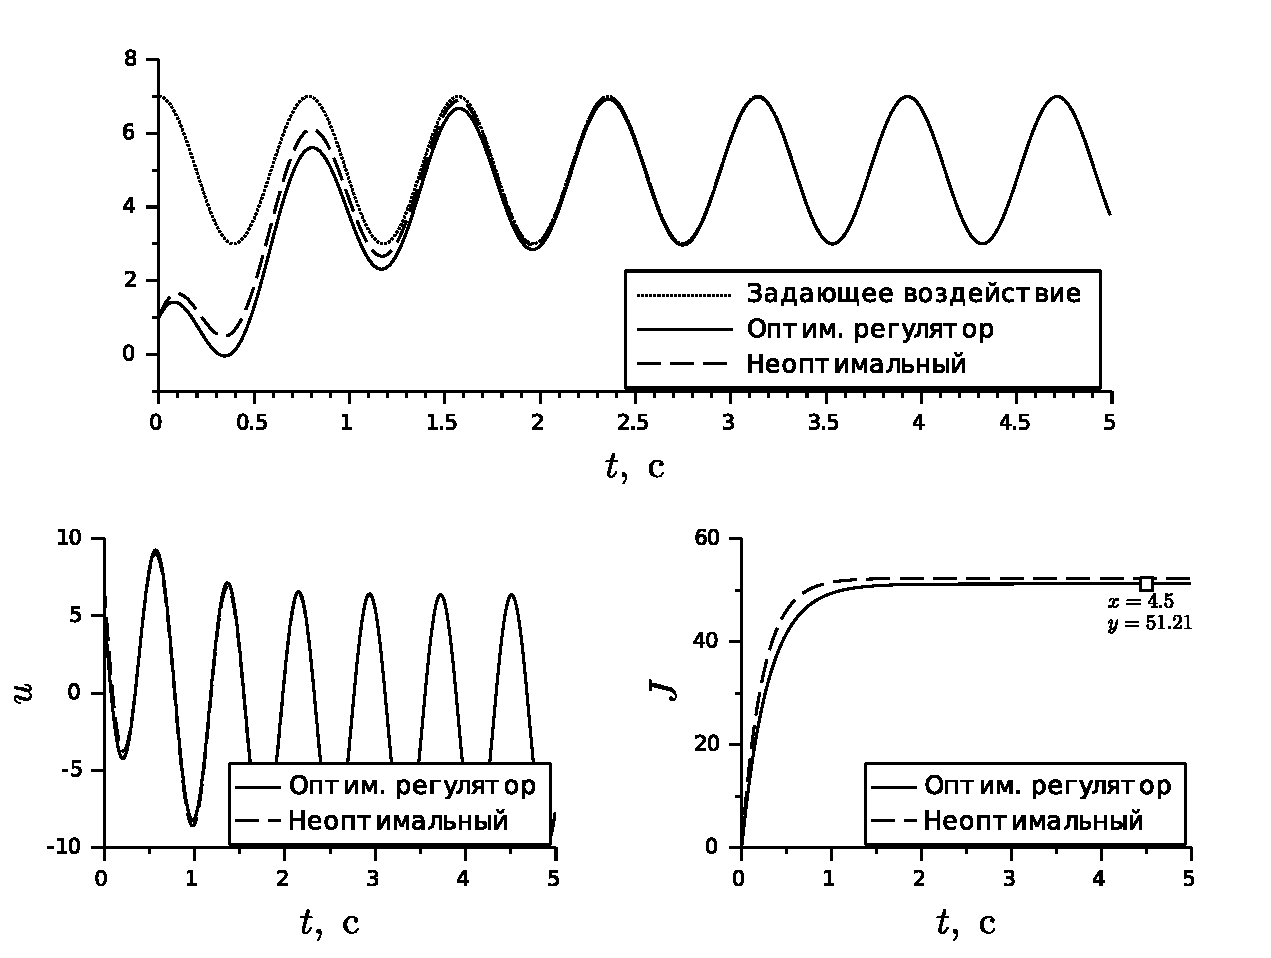
\includegraphics[width=\textwidth]{graphs.pdf}
    \vspace{0cm}
    \caption{Графики переходных процессов при оптимальном и неоптимальном регуляторах.}
    \label{img_graphs}
\end{figure}

\begin{figure}[h!]
    \centering
    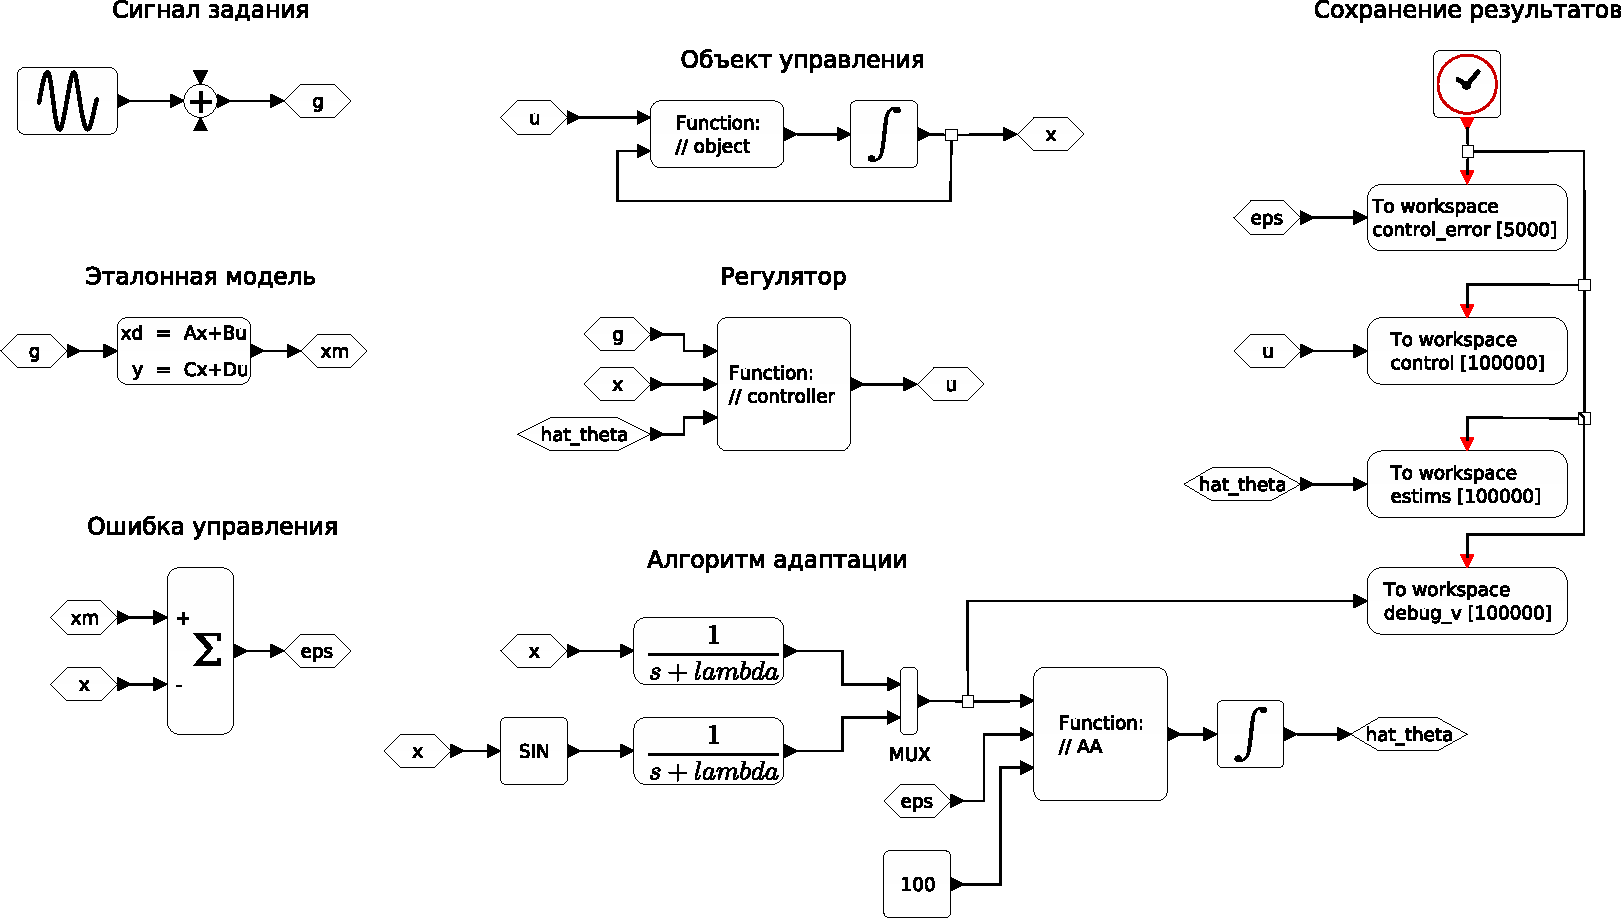
\includegraphics[width=0.95\textwidth]{modeling_scheme.pdf}
    \vspace{0.5cm}
    \caption{Схема моделирования рассматриваемой системы управления.}
    \label{img_modeling_scheme}
\end{figure}


\newpage


\section{Выводы по работе}
В~результате проделанной работы для заданного объекта управления был рассчитан регулятор, оптимальным образом решающий задачу его стабилизации с точки зрения минимизации значения конкретного критерия качества.
Последнее было проверено отклонением коэффициентов регулятора от их рассчитанных значений~--- как и следовало ожидать, установившееся значение критерия качества в таком случае оказалось больше, чем при оптимальном~$K$.
